\documentclass[11pt]{book}
\usepackage{fontspec}
\setmainfont{TeX Gyre Pagella}
\usepackage[margin=1in]{geometry}
\usepackage{xcolor}
\usepackage{tikz}
\usetikzlibrary{arrows.meta,shapes.geometric,shapes.misc}
\usepackage{amssymb}
\usepackage{enumitem}
\usepackage{titlesec}

\titleformat{\chapter}[display]{\bfseries\Large}{Sproll 10}{0.5em}{\Huge}
\titleformat{\section}{\bfseries\large}{\thesection}{0.6em}{}

\newenvironment{algorithmproc}[1]{\vspace{0.6em}\noindent\rule{\linewidth}{0.6pt}\\[0.2em]\textbf{How to Tell: #1}\\[0.3em]}{\\[0.2em]\noindent\rule{\linewidth}{0.6pt}\vspace{0.6em}}
\newenvironment{practicenow}{\vspace{0.6em}\noindent\rule{\linewidth}{0.6pt}\\[0.2em]\textbf{Practice Now}\\[0.3em]}{\\[0.2em]\noindent\rule{\linewidth}{0.6pt}\vspace{0.6em}}
\newenvironment{exercisebox}[1]{\vspace{0.8em}\noindent\rule{\linewidth}{0.6pt}\\[0.2em]\textbf{Exercises: #1}\\[0.3em]\begin{enumerate}[label=\arabic*., itemsep=0.4em]}{\end{enumerate}\noindent\rule{\linewidth}{0.6pt}\vspace{0.6em}}
\newenvironment{trythis}{\vspace{0.6em}\noindent\rule{\linewidth}{0.6pt}\\[0.2em]\textbf{Try This}\\[0.3em]}{\\[0.2em]\noindent\rule{\linewidth}{0.6pt}\vspace{0.6em}}
\newenvironment{summarybox}{\vspace{0.6em}\noindent\rule{\linewidth}{0.6pt}\\[0.2em]\textbf{What We Learned}\\[0.3em]}{\\[0.2em]\noindent\rule{\linewidth}{0.6pt}\vspace{0.6em}}

\begin{document}
\begin{titlepage}
\centering
\vspace*{1.4in}
{\Huge \textbf{SPROLL 10}}\\[0.5in]
{\huge Four Moves Make a World}\\[0.8in]
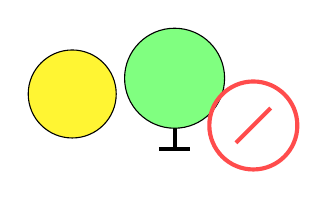
\begin{tikzpicture}
\filldraw[fill=yellow!80] (-1.3,0.3) circle (0.22in);
\draw[line width=1.5pt] (0,-0.4) -- (0,0.4);
\draw[line width=1.5pt] (-0.2,-0.4) -- (0.2,-0.4);
\filldraw[fill=green!50] (0,0.5) circle (0.25in);
\draw[line width=1.5pt, red!70] (1,-0.1) circle (0.22in);
\draw[line width=1.5pt, red!70] (0.78,-0.32) -- (1.22,0.12);
\end{tikzpicture}\\[0.8in]
{\Large The Sproll Curriculum}\\[0.2in]
{\large Cycle I: Pops --- Things, Differences, and Counting}
\end{titlepage}

\tableofcontents

\chapter*{Before You Begin}
\addcontentsline{toc}{chapter}{Before You Begin}

Nothing new is introduced in this workbook. Its only job is to put Pop, Refuse, Bind, and Collapse to work together, all four at once, building one small, complete world from nothing. If you can follow this construction and explain each step in your own words, you have finished the first cycle of the Sproll Curriculum.

\chapter{A Tiny World, Built Step by Step}

\section{Building the Scene}

Start with nothing on the page at all. Four events, in order, build a small scene.

First: Pop a sun. A yellow circle appears, chosen from among the things that could have been placed there.

Second: Pop a tree. A green shape appears beside the sun.

Third: Bind the tree to the ground. The tree is now connected to a line beneath it representing the ground, so that if the ground were to move, the tree would move with it, without the tree and the ground becoming the same thing.

Fourth: Refuse a second sun. Somewhere in the process, a second sun was considered and specifically rejected. It is not part of the finished scene, but it is part of the record: a genuine refusal, not an unmentioned absence.

\begin{center}
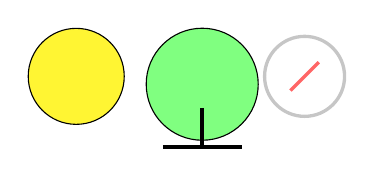
\begin{tikzpicture}
\filldraw[fill=yellow!80] (-1.3,0.6) circle (0.24in);
\filldraw[fill=green!50] (0.3,0.5) circle (0.28in);
\draw[line width=1.5pt] (0.3,0.2) -- (0.3,-0.3);
\draw[line width=1.5pt] (-0.2,-0.3) -- (0.8,-0.3);
\draw[line width=1.2pt, gray!45] (1.6,0.6) circle (0.2in);
\draw[line width=1.2pt, red!60] (1.42,0.42) -- (1.78,0.78);
\end{tikzpicture}
\end{center}

\begin{algorithmproc}{Reading a Construction}
To understand any constructed scene in this curriculum, list its events in order: which Pops happened, which Refusals happened, which Binds connect which parts. The finished picture is only the final Collapse of that full history under a particular rule; the history itself is what actually explains why the picture looks the way it does.
\end{algorithmproc}

\begin{practicenow}
Using only the four moves from this workbook, plan a tiny scene of your own (at least two Pops, one Bind, and one Refuse). Write out your plan as an ordered list of events before drawing or building anything.
\end{practicenow}

\begin{exercisebox}{Section 1.1}
\item List the four events used to build the sun-and-tree scene, in order, and name which primitive action each one is.
\item Explain why the refused second sun is part of this world's history even though it is not part of the finished picture.
\item Challenge: could the same finished picture (sun, tree, ground) have been built using a different order of events, or even a different set of events entirely? Try to describe an alternative construction that reaches the same picture.
\end{exercisebox}

\chapter{Looking at the Same World Two Ways}

\section{Two Honest Collapses of One Scene}

Apply the ordinary picture rule to this history, and you get exactly the drawing shown above: a sun, a tree, and the ground, connected. Apply a different rule instead, one that counts only the Pop events, ignoring Binds and Refusals entirely, and you get a plain number: two, one Pop for the sun and one Pop for the tree.

Both are completely correct Collapses of the exact same underlying history. Neither is more real than the other. This is the same lesson from Sproll 06 and Sproll 07, now applied to a full little world rather than to a single shape or a short history.

\begin{trythis}
Take the scene you planned in the Practice Now above. Collapse it under the ordinary picture rule (draw or build it) and separately under the count-only-Pops rule (state the number). Confirm both results are correct descriptions of the same construction.
\end{trythis}

\begin{exercisebox}{Section 2.1}
\item State a third Collapse rule you could apply to the sun-and-tree history, besides the picture rule and the count-only-Pops rule, and give its result.
\item Explain why ``the picture'' and ``the number of Pops'' can both be correct answers to ``what is this history,'' despite looking nothing alike.
\item Challenge: is there a Collapse rule for this history that would give a wrong or nonsensical answer? What would make a rule inappropriate for a particular history?
\end{exercisebox}

\chapter{What Four Moves Can Do}

\section{The Whole Cycle, in Four Actions}

Pop commits to one option among several, so that a fact now exists that did not exist before. Refuse deliberately marks an option as not chosen, while leaving it fully visible and nameable, never simply erasing it. Bind connects two things so that they depend on each other, without ever merging them into one. Collapse applies a chosen rule to a constructed history and produces a result, a picture, a count, or anything else the rule is built to produce.

Every workbook in this cycle, from Sproll 00's first careful look at telling one thing from another, through today's small constructed world, has been building toward exactly these four actions and nothing more. Ordinary counting, ordinary sorting, ordinary equality, and even the idea of a whole built from parts, all of it has come from combinations of just these four moves.

\begin{summarybox}
A world, no matter how small, can be built entirely from four actions: Pop, Refuse, Bind, and Collapse. The same constructed history can be examined under different Collapse rules, producing different, equally correct results. This is the complete toolkit Cycle I set out to build, and every later cycle in this curriculum uses these same four moves, never adding a fifth.
\end{summarybox}

\begin{exercisebox}{Section 3.1}
\item In your own words, define each of the four primitive actions from this curriculum: Pop, Refuse, Bind, Collapse.
\item Build or describe your own small world using all four actions at least once, and write out its full history in order.
\item Challenge: can you think of any action you might want to perform on a constructed world that does NOT fit into one of these four categories? If so, describe it; if not, explain why you think these four are enough.
\end{exercisebox}

\chapter*{That Is Cycle I}
\addcontentsline{toc}{chapter}{That Is Cycle I}

Ten workbooks ago, this curriculum began by asking whether one thing could be told apart from another. It now ends its first cycle with a complete toolkit for building, refusing, connecting, and observing an entire small world. Every later cycle in the Sproll Curriculum builds directly on top of these four actions; none of them are ever replaced.

The next cycle asks a new kind of question. Instead of building one history at a time, what happens when many things exist together, and a rule decides which of them belong and which do not? Every world, it turns out, needs a boundary: something to decide what is inside and what is outside. That is where Cycle II, Rules: Making Little Worlds, begins.

\chapter*{For Parents and Teachers}
\addcontentsline{toc}{chapter}{For Parents and Teachers}

This workbook is Cycle I's consolidation and introduces no new formal content; its purpose is to demonstrate that a child who has worked through Sprolls 00 through 09 can now read, plan, and explain a small constructed world using all four primitive actions correctly and in combination. A reasonable completion check is simply asking the child to narrate this workbook's sun-and-tree scene back in their own words, correctly identifying which event was a Pop, which was a Refuse, and which was a Bind, and to explain, in some form, why the picture and the Pop-count are both legitimate ways of looking at the same history.

Cycle II shifts the curriculum's attention from constructing a single history to reasoning about membership and rules across many possible Pops at once, laying the groundwork for sets, predicates, and eventually the idea of deliberately changing an admissibility rule itself, introduced gradually and without formal vocabulary until much later in the series.

\end{document}
